\documentclass[a4paper,man,natbib,floatsintext,donotrepeattitle]{apa6}
\usepackage[english]{babel}
\usepackage[utf8x]{inputenc}
\usepackage{amsmath}
\usepackage{graphicx}
\usepackage{xcolor}
\usepackage[draft,inline,nomargin,index]{fixme}
\usepackage[hidelinks]{hyperref}
\usepackage{verbatim}
\usepackage{nameref}
\usepackage{lineno}
\usepackage{amsfonts}
\usepackage{booktabs}
\usepackage{siunitx}
\usepackage[symbol]{footmisc}
\usepackage{dirtytalk}

% for comments
\usepackage{todonotes}

% adding an epigraph
\usepackage{epigraph}

% changing epigraph width
\setlength{\epigraphwidth}{0.75\textwidth}

% right-align epigraph
\renewcommand{\textflush}{flushright}

% adapting dois to follow APA6
\renewcommand{\doiprefix}{}
\newcommand{\doi}[1]{\href{https://doi.org/#1}{https://doi.org/#1}}

% new command for Donny's comments
\newcommand{\DWcomment}[2][inline]{\todo[author=DW, color=red!20, #1]{#2}}

% enabling line numbers
\linenumbers

% making footnotes in arabic style
\renewcommand{\thefootnote}{\arabic{footnote}}

\title{Pragmatism should not be a substitute for statistical literacy, a commentary on \cite{albers_credible_2018}}

\shorttitle{Pragmatism versus parsimony}

\threeauthors{Ladislas Nalborczyk}{Paul-Christian Bürkner}{Donald R. Williams}

\threeaffiliations{Univ. Grenoble Alpes, CNRS, LPNC, 38000, Grenoble, France \\ Department of Experimental Clinical and Health Psychology, Ghent University, Belgium}{Department of Psychology, University of Münster, Germany}{Animal Behavior Graduate Group, University of California, United States}

\abstract{Based on the observation that frequentist confidence intervals and Bayesian credible intervals sometimes happen to have the same numerical boundaries (under very specific conditions), \cite{albers_credible_2018} proposed to adopt the heuristic according to which they can usually be treated as \textit{equivalent}. We argue that this heuristic can be misleading by showing that it does not generalise well to more complex (realistic) situations and models. Instead of pragmatism, we advocate for the use of parsimony in deciding which statistics to report. In a word, we recommend that a researcher interested in the Bayesian interpretation simply reports credible intervals.}

\keywords{Bayes, Bayesian statistics, confidence interval, credible interval}

\authornote{Correspondence concerning this article should be addressed to Ladislas Nalborczyk, Laboratoire de Psychologie et Neurocognition, Univ. Grenoble Alpes, 1251 avenue centrale, 38058 Grenoble Cedex 9, France. E-mail: \href{mailto:ladislas.nalborczyk@univ-grenoble-alpes.fr}{\nolinkurl{ladislas.nalborczyk@univ-grenoble-alpes.fr}}.}

\begin{document}

% defining a new command for counting words
\newcommand{\quickwordcount}{
  \immediate\write18{texcount -1 -sum -merge main.tex > \jobname-words.sum}
  \input{\jobname-words.sum}words
}

\maketitle

Wordcount: This document contains \textbf{\quickwordcount}.

\newpage

% restoring section numbering (disabled by the apa template)
\setcounter{secnumdepth}{3}

\epigraph{If a thing can be done adequately by means of one, it is superfluous to do it by means of several; for we observe that nature does not employ two instruments where one suffices.}{\textit{Aquinas, [BW], p.129}}

\section{Context}

\cite{albers_credible_2018} offered a very concise discussion of the frequentist versus Bayesian debate from a pragmatic perspective, and suggested refreshing and thought-provoking ideas on this perpetuating debate.

The main line of reasoning of \cite{albers_credible_2018} seems to be the following: as frequentist confidence intervals and Bayesian credible intervals sometimes happen to be similar, we can usually interpret them the same way. More precisely, they argue that because confidence intervals and credible intervals do sometimes have the same numerical boundaries (and because when they do, they have similar consequences on the inference being made), then, from a pragmatic perspective, they should be treated as \textit{equivalent}.

However, we argue that i) the situations presented in \cite{albers_credible_2018} are overly simplistic and actually quite rare, ii) even in the sparse situations where the numerical boundaries of the intervals are identical, the inference that can be made from each interval is not identical, and that iii) pragmatism comes with its own pitfalls, that could easily be avoided by using parsimony instead as a guiding principle, and by relying on statistical literacy rather than  misguided and misleading heuristics.

\section{Rebuttals}

%\subsection{Restating Bayes theorem, a tautology}

%From a broad perspective, outlining that confidence intervals are usually equivalent to credible intervals when using non-informative priors is akin to simply rephrasing Bayes theorem, which states that the posterior is proportional to the likelihood times the prior, that is:

%$$ posterior \propto likelihood \times prior $$

%From this theorem, we can deduce that if the prior is non-informative, then the posterior can be equated with the likelihood. It follows that frequentist estimates (who depends only on the likelihood) can be equated with Bayesian estimates (that are obtained from the posterior distribution) when uninformative priors are used. In other words, frequentist statistics can be conceived as a particular case of Bayesian statistics. Given that this conclusion is a strict deduction from Bayes theorem, we feel that rhetorical demonstrations and numerical simulations aiming at demonstrating this equality would add very little to the current state of knowledge.

\subsection{Conditioning on nonsense}

The debate between the frequentist and the Bayesian schools of inference has been firing for many decades and we do not wish to reiterate all the arguments here (we refer the interested reader to the introduction of \citealp{albers_credible_2018}).

Bayesian statistics rest on the use of Bayes' rule, which states that:

$$ p(\theta|y) \propto p(y|\theta) \times p(\theta) $$

In other words, the posterior probability of some parameter (or vector of parameters) $\theta$ is proportional to the product of its prior probability $p(\theta)$ and the likelihood $p(y|\theta)$. Noteworthy here is that the posterior probability $p(\theta|y)$ can be interpreted as a \textit{conditional} probability, \textit{given} the data \textit{and} the model (including the prior information).

 This highlights a first undesirable consequence of \cite{albers_credible_2018}'s proposal. Using confidence intervals (or credible intervals with flat priors) to make probability statements can lead to nonsensical situations. For instance, let's say you're fitting a simple linear regression model to estimate the average reaction time in some cognitive task\footnote{Which is given by the intercept of the model, if no predictor is included, or if these predictors are centred.}. Using a confidence interval to make a probability statement (under the pretence that it is numerically similar to a credible interval) is akin to implicitly assuming a uniform prior over the reals. It means assuming that every value between $-\infty$ and $\infty$ are equally plausible, including negative values. This obviously does not make sense when we are dealing with reaction times, proportions, scales scores, most physical measurements (e.g., weight, height), or anything else that has a restricted range of definition.
 
 Further, there are examples where numerically equivalent intervals do not necessarily reflect the most probable parameter values (given all available information), but could still have valid frequentist properties. That is, while both Bayesian and frequentist intervals could have nominal coverage probabilities \citep{albers_credible_2018}, the additional requirement for (meaningful) probabilistic inference is compatibility with previous information. Here Bayesian probability is not inherently subjective. Rather, in addition to the data, the probabilities are also conditional on all assumptions including the prior distribution. To make this point, we use a recent example from a registered replication report \citep{verschuere_registered_2018}. The original effect was reported as $d$ = 1.45, 95\% [0.29, 2.61] \citep{mazar_dishonesty_2008}. Following the argument of \cite{albers_credible_2018}, we could state there is a 50\% chance the effect is greater than 1.45. Although this would be mathematically correct for the posterior distribution \citep{gelman_p_2013}, this does not mean it accurately reflects the most probable values. Indeed, based on the priming literature, it would be unreasonable to make such a probability statement. On the other hand, we could envision such a wide interval (Bayesian or frequentist) covering the population value 95\% of the time. Thus, interpretive exchangeability is not a given and can lead to misleading inferences when conditioning on nonsense.

\subsection{On the wrong use of credible intervals}

While it is legitimate to use confidence intervals as tests (these can be considered as regions of significance), credible intervals cannot be used to reject a specific value. As explained in \cite{morey_fallacy_2015}, testing a specific value of interest in a Bayesian framework requires that this specific value is assigned a non-zero probability a priori. Using credible intervals as a way of rejecting a null value would be similar to doing NHST, without controlling error rates (which is usually not desirable).

For this reason, we feel that every proposal going in the direction of more fuzziness in the distinction between different kinds of intervals is misleading and should be rejected. To put it more clearly (and as it will become clear by the end of the current paper), using a confidence interval as a credible interval or using a credible interval as a confidence interval is "simply wrong" (\citealp{berger_bayes_2006}, quoted in \citealp{morey_fallacy_2015}).

\subsection{Risks of conceptual overfitting: the case against pragmatism}

It is usually not enough for two entities to have the same numerical values to conclude that we can interpret them the same way. It is even less sufficient to allow for the conclusion that they have the same characteristics. As an analogy, we discuss below a comparison of the concepts of mass and weight.

Both measures can sometimes (under particular conditions of gravitational acceleration) give similar numerical estimations of a physical phenomenon. However, even in this situation, they do have very different meanings. Mass is a measure of the amount of matter an object is made up of (that we can express in kilograms), while weight refers to the force exerted on an object by gravity (expressed in newtons). The relation between weight ($W$), mass ($M$) and gravitational acceleration ($G$) is given by the following equation:

$$ W = M \times G $$

As an example, the weight of an object of 100kg on Earth is approximately equals to $100 \times 9.8 = 980 \text{N}$. However, the weight of an object of 100kg on the Moon is approximately equals to $100 \times 1.622 = 162.2\text{N}$. Let's now consider an environment $E$ in which $G = 1$. In this environment, $W$ is equals to $M$ and a pragmatical agent would conclude that both concepts are identical, because they seem to describe a similar aspect of the world. However, this numerical equivalence under restricted conditions does not warrant ontological equivalence (i.e., it's not because two things have the same numerical value in very specific situations that they \textit{are} the same thing, or that they will have the same numerical value in other situations). As a consequence, using mass as a proxy for weight would lead to identical numerical estimates in a very limited range of situations (actually in precisely one situation, i.e., when $G = 1$), but would lead to different numerical estimations in all the other situations (i.e., the situations in which $G$ differs from exactly 1). To put it simply, the belief that $W = M$ would lead to erroneous predictions in every situation except the one where this belief was formed (a concept also known as overfitting).

In a similar way, a frequentist confidence interval carries information about the hypothetical sampling distribution of the statistics under study (e.g., the mean), while a Bayesian credible interval is a way of summarising the posterior distribution. These are two very different things, that can, occasionally, happen to be numerically equivalent.

As discussed previously, \cite{albers_credible_2018} focused on very simplistic situations (the estimation of the mean of an unimodal distribution and the estimation of a proportion) to illustrate their point, without considering the generalisability of the claim. Similarly to the person living in the environment with $G = 1$, we are afraid that the heuristic according to which confidence intervals can be interpreted as credible intervals will lead to disappointment in most situations\footnote{One should also consider the risk that the target paper becomes a reference for justifying the Bayesian interpretation of confidence intervals in situations that do not warrant this interpretation.}. We now move to a discussion of two concrete examples examining the generalisability of the heuristic suggested by \cite{albers_credible_2018} in regards to the coverage properties (and the numerical boundaries) of confidence intervals and credible intervals.

\subsection{Frequentist properties of Bayesian credible intervals}

\subsubsection{A simple regression example}

In Figure \ref{fig:coverage}, we present some simulation results showing that Bayesian credible intervals (obtained with weakly informative priors) do have the same properties as frequentist confidence intervals in the case of a simple regression model. Indeed, on repeated sampling, X\% of the constructed intervals will contain the population value of $\theta$ (as expressed by the coverage proportion displayed in Figure \ref{fig:coverage}).

\begin{figure}[H]
  \caption{Coverage properties of Bayesian credible intervals when using weakly informative priors. Blue vertical credible intervals represent intervals that "missed" the population value of the parameter (whose value is represented by the horizontal dashed line), while grey intervals represent intervals that contained the population value. Note: for readability, only the first 100 simulations are plotted.}
  \centering
  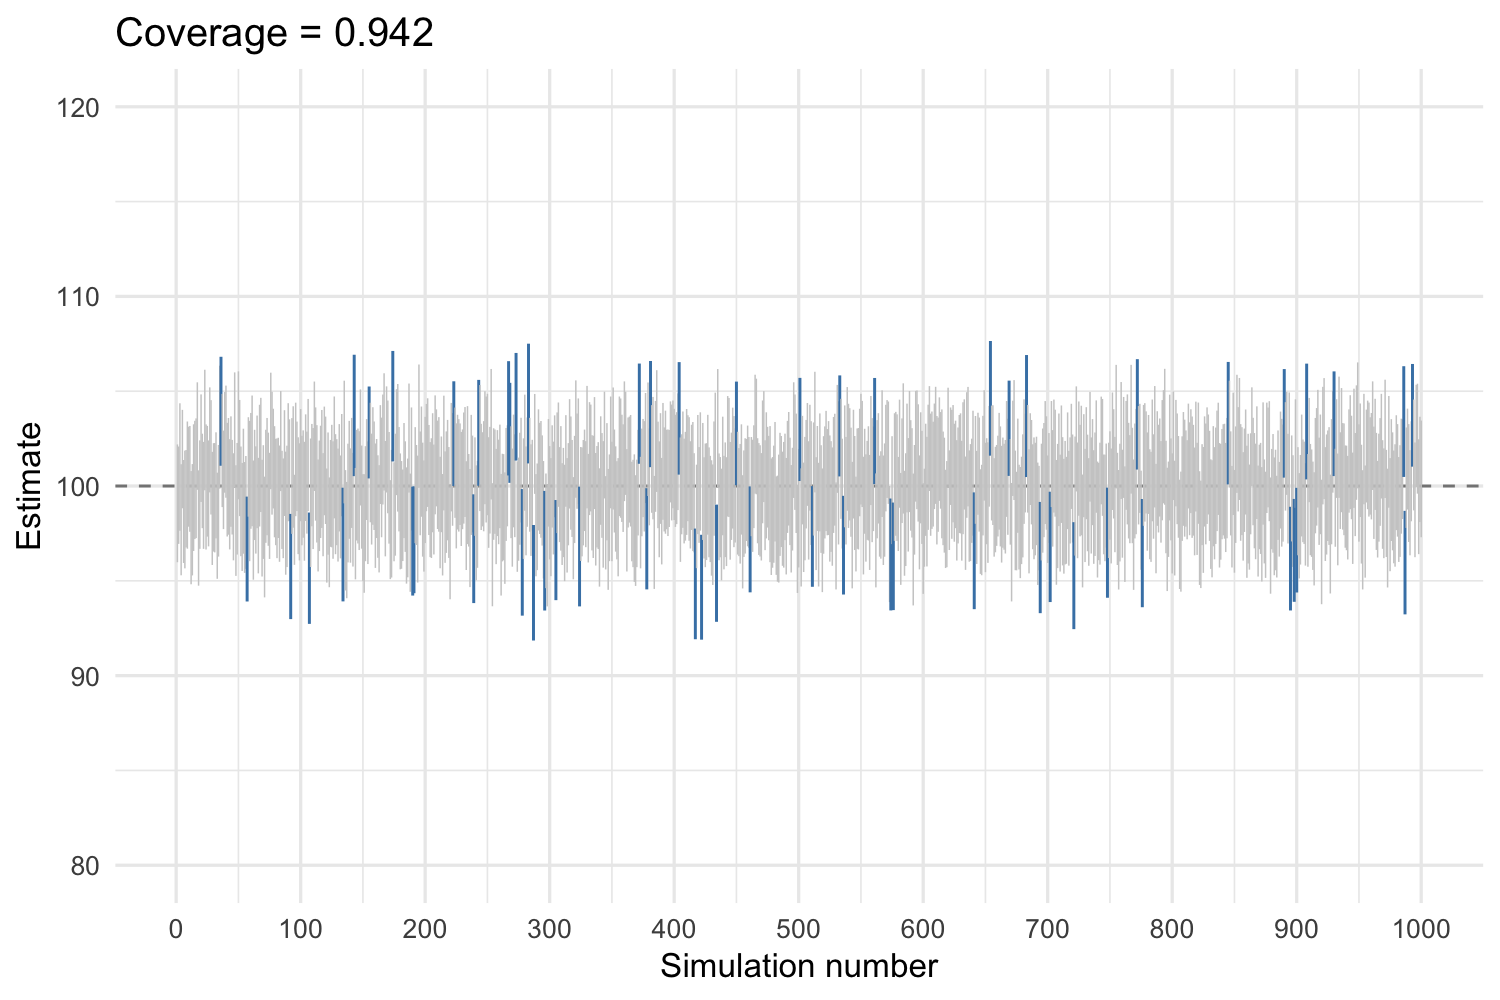
\includegraphics[width=0.8\textwidth]{coverage1.png}
  \label{fig:coverage}
\end{figure}

Bayesian credible intervals with non-informative or weakly informative priors may have the same frequentist characteristics as confidence intervals, but also allow for conditional probability statements (e.g., given the prior and the information contained in the data, we can say that there is a X\% probability that the population value of $\theta$ lies in the interval)\footnote{Although, as we discussed earlier, this probability statement, while valid, makes little sense knowing that it is conditional on all possible values being equally likely a priori.}.

Therefore, in simple situations, the principle of parsimony would lead to use and report the most inclusive (general) statistics. In contrast to what \cite{albers_credible_2018} advocate, we thus suggest that the researcher interested in the Bayesian interpretation should use and report Bayesian statistics along with sensitivity analyses, with non-informative, weakly informative and informative priors (whose information might come from subject matter knowledge).

\subsubsection{What about more complex models?}

In this section, we report simulation results of the coverage properties of both confidence and credible intervals around the amount of heterogeneity $\tau$ in random-effects meta-analysis models.

The effect sizes to be combined in meta-analyses are often found to be more variable that it would happen because of sampling alone. The usual way to take into account this heterogeneity is to use random-effects models (also known as multilevel models). Several methods have been proposed to obtain confidence intervals around the point estimate of $\tau$ in such models (for a discussion, see \citealp{williams_bayesian_2018}). The method developed by \cite{paule_consensus_1982} and implemented in the \texttt{metafor} package \citep{viechtbauer_conducting_2010} guarantees nominal coverage probabilities of confidence intervals computed with this method, even in small samples, given that model assumptions are satisfied. Below we compare the coverage properties of confidence intervals (computed with this method) and credible intervals for a simple random-effects meta-analysis model of 6 studies, with a population value of $\tau = 0.1$ (see code in supplementary materials for more details).

\begin{figure}[H]
  \caption{Coverage properties of 95\% confidence intervals and 95\% credible intervals for recovering the amount of heterogeneity in random-effects meta-analysis models. Note: for readability, only the first 100 simulations are plotted.}
  \centering
  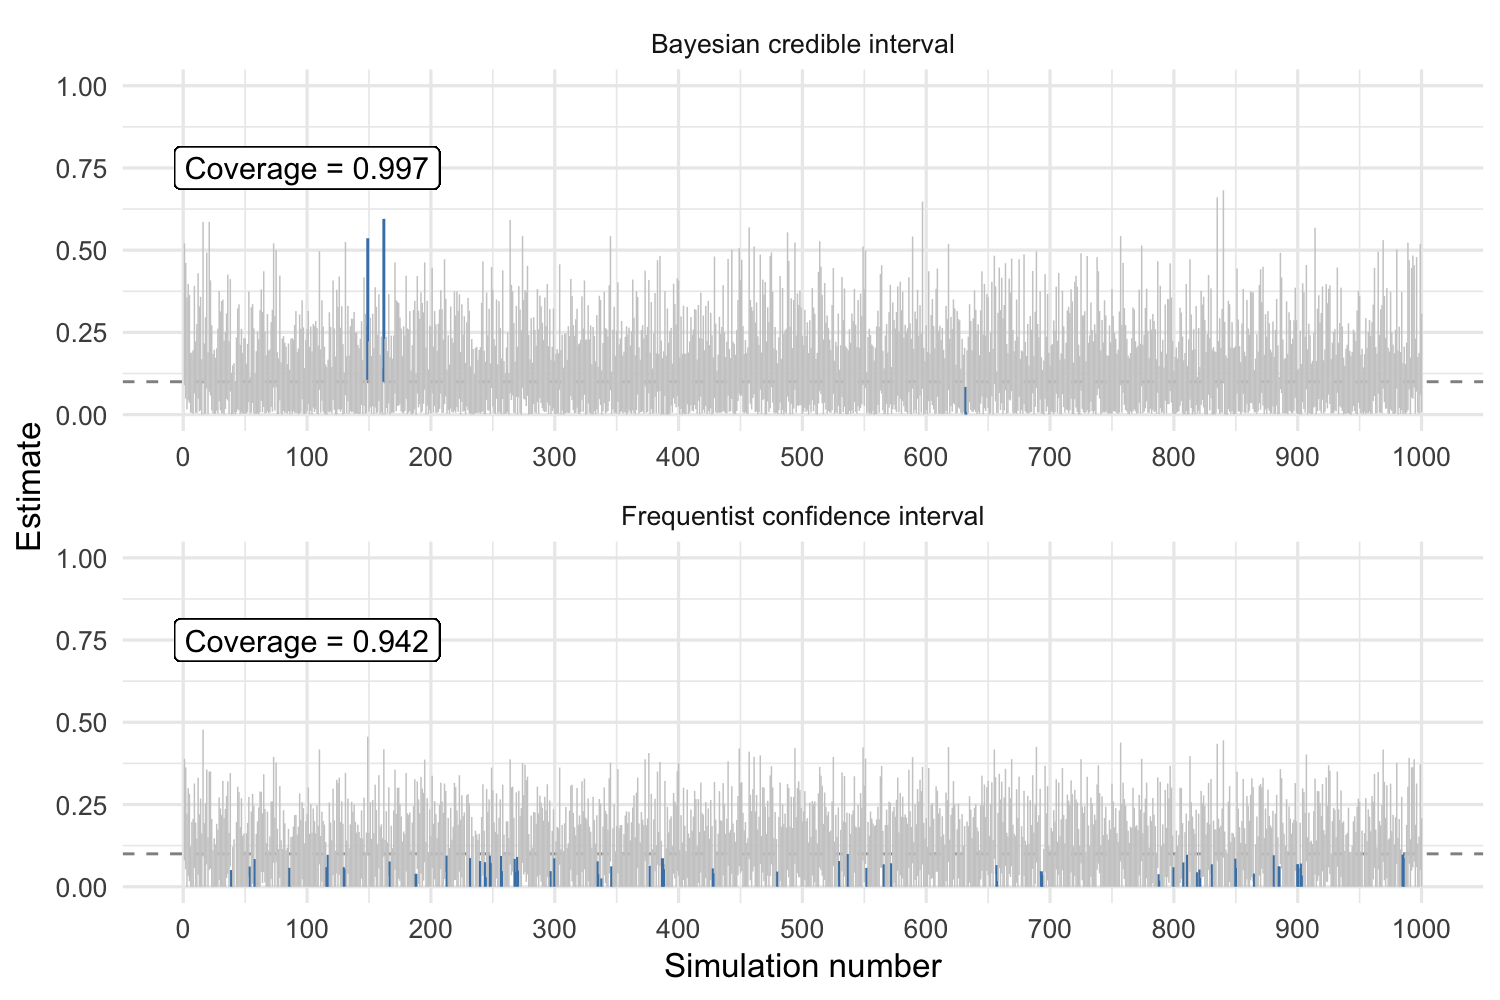
\includegraphics[width=0.8\textwidth]{coverage2.png}
  \label{fig:coverage2}
\end{figure}

As shown in Figure \ref{fig:coverage2}, the coverage proportion of confidence intervals is close to the nominal 95\% value. However, the credible intervals (wider than the confidence intervals) appear to contain the population value of $\tau$ in almost all 10.000 simulations, resulting in a coverage proportion close to 1.

Thus, in contrast to what \cite{albers_credible_2018} claimed, it appears that even when using non-informative priors (we used $\tau \sim \mathrm{HalfCauchy}(1000)$), the numerical boundaries as well as the coverage properties of confidence intervals and credible intervals can differ considerably. More generally, we feel that using simplistic examples to make general claims is highly problematic in that there is no guarantee that this generalises well to more complex models.

\subsection{Differences matter}

\cite{albers_credible_2018} write: "In the present paper, we have demonstrated by means of various examples that confidence intervals and credible intervals, in various practical situations, are very similar and will lead to the same conclusions for many practical purposes when relatively uninformative priors are used".

Contrary to what the authors postulate, differences between confidence intervals and credible intervals are observable in an incredible large variety of situations (actually, all but one). For instance (but non exhaustively), i) when samples are small, ii) when the space of the outcome is multi-modal or non-continuous, iii) when the range of the outcome is restricted, or iv) when the prior is at least weakly informative. Combining these four possibilities, we argue that confidence intervals and credible intervals actually almost never give similar results. Moreover, as we previously demonstrated, numerical estimates can be similar, but it does not entail that the conclusion we can draw from it (i.e., the inference being made) should be similar.

%\subsection{Drawbacks of extreme pragmatism}

%In this section, we want to highlight what appears to us as a fallacious argument\footnote{We recognise that the fallacy comes from the imperfect correspondence between confidence intervals and credible intervals.}. As a reminder, \cite{albers_credible_2018} argue that because confidence intervals and credible intervals do sometimes have the same numerical values (and because when they do they have similar consequences on the inference being made), then, from a pragmatic perspective, they should be treated as \textit{equivalent}. Thus, we could use confidence intervals instead of (or in addition to) credible intervals.

%This argument seems to be of the following form: "Because $A$ can sometimes be interpreted as $B$, then we should use $A$ instead of (or in addition to) $B$". Does it mean that if astrology sometimes gives the same results as personality tests, we should use astrology instead of (or in addition to) personality tests ?

In the previous sections, we discussed why we think the logic of the argument presented in \cite{albers_credible_2018} can be misleading. In the following, we suggest an alternative to pragmatism which does not preclude statistical literacy.

\section{An alternative to pragmatism}

\subsection{Applying parsimony in scientific and statistical practise}

\cite{albers_credible_2018} write: "By recognizing the near-equivalence between Bayesian and frequentist estimation intervals in ‘regular cases’, one can benefit from both worlds by incorporating both types of analysis in their study, which will lead to additional insights."

Confidence intervals can sometimes (i.e., under specific conditions) be identified with a special case of credible intervals for which priors are non-informative. Thus, one could ask, in consideration of the parsimony principle, why reporting redundant statistics? Would not it be easier to use the more general and flexible case? The parsimonious stance that we adopt here lead to the conclusion that the researcher interested in one specific interpretation should report the statistics that corresponds to this goal\footnote{Obviously, it is perfectly legitimate to be interested in several goals, but these goals should be clearly stated as such, and pursued using appropriate tools.}. If a researcher is interested in the sampling distribution of the statistics under study (or in reaching a nominal coverage proportion), s$\cdot$he should report confidence intervals. If s$\cdot$he is rather interested in making conditional probability statements from the data, then s$\cdot$he should report credible intervals (or ideally, the full posterior distribution).

\subsection{A brief note on the frequentist properties of Bayesian procedures}

\cite{albers_credible_2018} quote \cite{bayarri_interplay_2004} that wrote: "Statisticians should readily use both Bayesian and frequentist ideas".

We could not agree more with this statement. In addition, we recognise that both statistical traditions have their own advantages and drawbacks, and have been built to answer somehow different questions. Therefore, we feel that pretending that a statistic issued from one school of inference can be interpreted as a statistic issued from another school because they sometimes (under very restricted conditions) give the same numerical estimates is confusing and misleading.

\section{Conclusions and practical recommendations}

Given the limitations of the pragmatic perspective offered by \cite{albers_credible_2018} and the potentially harmful consequences of the heuristic they argued for, we rather suggest to use parsimony as a guiding principle in deciding which statistics to use and to report.

In order to warrant the Bayesian interpretation of frequentist confidence intervals, each confidence interval should be accompanied by a Bayesian credible interval. However, reporting credible intervals aside from confidence intervals in order to be sure that the confidence interval can be interpreted as a credible interval makes little sense to us, as it would lead to reporting redundant intervals (when they are identical). For the sake of parsimony, we therefore recommend that a researcher interested in the Bayesian interpretation of an interval simply reports credible intervals along with sensitivity analyses (or that a researcher interested in the coverage properties of confidence intervals simply reports confidence intervals). In brief, we argue for ecumenism and we think pragmatism should not be a substitute for statistical literacy. 

As \cite{hoekstra_improving_2018}, we believe that "the more pragmatic approach in which philosophically unsound interpretations of CIs are permitted and even endorsed is unhelpful, and should be replaced by a more principled one. If students are to learn a certain statistical technique, expecting from statistics teachers to guard them against quick-and-dirty versions seems very reasonable indeed".

\section{Data Accessibility Statement}

Reproducible code and figures are available at: \href{https://osf.io/nmp6x/}{\nolinkurl{https://osf.io/nmp6x/}}.

\section{Competing Interests}

The authors have no competing interests to declare.

\section{Author Contribution}

LN wrote a first version of the manuscript and conducted the simulations for the regression example. DW wrote a part of the paper and conducted the simulations for the meta-analysis example. DW and PB critically commented on various versions of the manuscript. All authors contributed to writing of the final manuscript.

\section{Acknowledgements}

We thank Antonio Schettino and Ivan Grahek for helpful comments on a previous version of this manuscript.

\bibliography{parsimony}

%\setlength{\parindent}{-0.5in}
%\setlength{\leftskip}{0.5in}
  
\end{document}
